\section{Design}
In questa sezione infine si trovano gli UXDiagram, ovvero i diagrammi che mostrano le schermate visibili agli utenti del sistema.
\subsection{UXDiagram}
Si suppone che la Homepage sia un landmark.
\subsubsection{UX per un ospite}
\begin{center}
 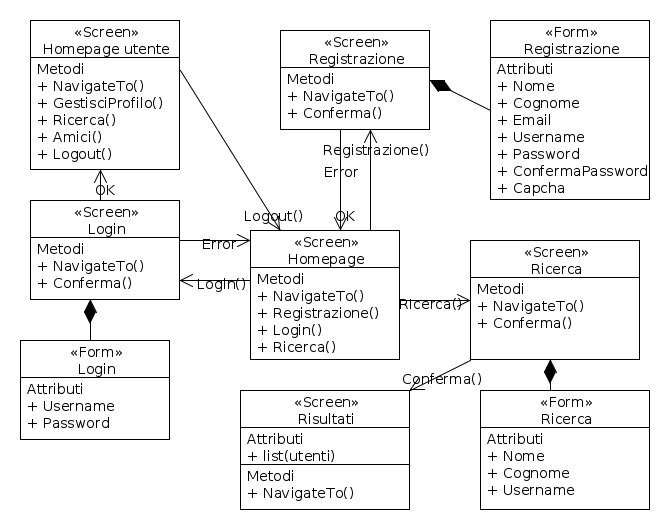
\includegraphics[width=1\columnwidth]{uxaccesso.png}
\end{center}
\pagebreak
\subsubsection{UX per un utente registrato}
Si suppone che la homepage dell'utente sia un landmark limitatamente agli utenti registrati e che si possa effettuare il logout da qualunque pagina
\begin{center}
 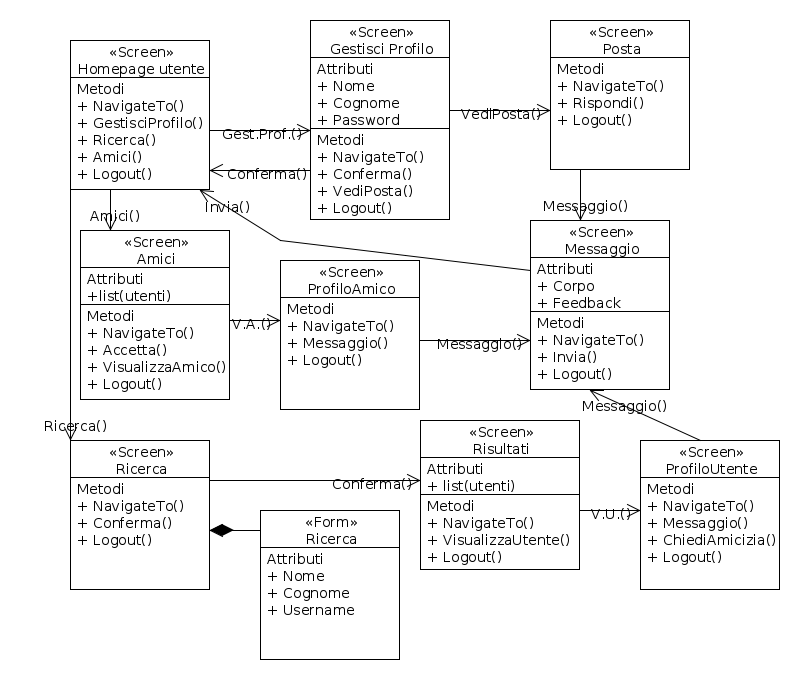
\includegraphics[width=1\columnwidth]{uxutente.png}
\end{center}
\pagebreak
\subsubsection{UX per un amministratore}
Questo UX Diagram contiene solo le funionalità esclusive dell'amministratore per motivi di leggibilità
\begin{center}
 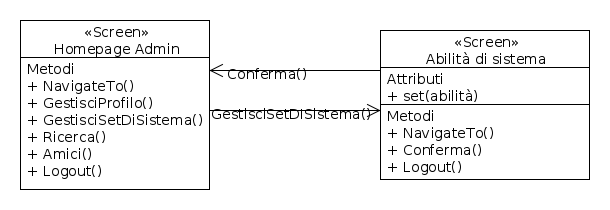
\includegraphics[width=1\columnwidth]{uxadmin.png}
\end{center}